\section{Parameter Effects}

The effects of the parameters on the model function are straightforward and can be read directly from the previous section.
In summary, the parameter $p_x$ changes the height of the branches $\B$ and $\D$ at their left border, where a lower $p_x$ means a higher value of the model function at these points.
In the previously defined notation, this is written as $\AL_{\B}^-$.
This notation is defined in \Cref{sec:yunus.param.effects}.
The parameter $p_y$ changes the offset of branches $\A$ and $\C$, so it moves the whole branches in contrast to $p_x$.
A higher $p_y$ means a higher offset and it is written as $\AW_{\A}^+$.


\Cref{fig:final.param.effects.px,fig:final.param.effects.py} illustrate these parameter effects.
Both figures show the model function for three parameter combinations, where either $p_x$ or $p_y$ is fixed and the other parameter is changed.
The model function is colored according to the changed parameter, blue is for the lowest value and red is for the highest value.
\Cref{fig:final.param.effects.px} illustrates the effect of $p_x$.
You can see, how the left borders of branches $\B$ and $\D$ are lower for higher values of $p_x$.
\Cref{fig:final.param.effects.py} illustrates the effect of $p_y$.
Here one can see, how the whole branches $\A$ and $\C$ move up for higher values of $p_y$.

\begin{figure}
    \centering
    \begin{subfigure}{0.4\textwidth}
        \centering
        \includegraphics[width=\textwidth]{60_Final/ParameterEffects/p_x/illustration.png}
        \caption{$p_x$}
        \label{fig:final.param.effects.px}
    \end{subfigure}
    \begin{subfigure}{0.4\textwidth}
        \centering
        \includegraphics[width=\textwidth]{60_Final/ParameterEffects/p_y/illustration.png}
        \caption{$p_y$}
        \label{fig:final.param.effects.py}
    \end{subfigure}
    \caption{Illustration of Parameter Effects}
\end{figure}

\Cref{tab:final.def.parameters.effects} list the effects of parameters $p_x$ and $p_y$ in a table, like also done for the original model in \Cref{sec:yunus.param.effects}.
Additionally, the parameter effects of the parameters in the original model are listed for comparison.
This gives a nice overview of which characteristics of the original model function are necessary for the observed bifurcation patterns.
Especially it shows, which parameter effects are not necessary.
For example, the effect $\AMi_{\B}^{L-}$ cannot even be fabricated in this model since branches $\B$ and $\D$ are linear and do not have a local minimum.
Also the effect $\AB_{\B\C}^L$, which is the movement of the borders between branches $\B$ and $\C$ (and $\D$ and $\A$ respectively), is not necessary.

\begin{table}
    \centering
    \begin{tabular}{|c||c|c||c|c|} \hline
        Combined         & $E_0$            & $\chi_0$          & $p_x$        & $p_y$          \\ \hline \hline
        $\AL_{\B}^{-}$   & $\AL_{\B}^{-}$   &                   & $\AL_{\B}^-$ &                \\ \hline
        $\AMi_{\B}^{L-}$ & $\AMi_{\B}^{L-}$ & $-\AMi_{\B}^{+}$  &              &                \\ \hline
        $\AW_{\A}^{+}$   &                  & $\AW_{\A}^{+}$    &              & $\AW_{\A}^{+}$ \\ \hline \hline
        $\AB_{\B\C}^{L}$ &                  & $\AB_{\B\C}^{L}$  &              &                \\ \hline
                         & $\AB_{\A\B}^{R}$ & $-\AB_{\A\B}^{L}$ &              &                \\ \hline
    \end{tabular}
    \caption{Comparison of Parameter Effects}
    \label{tab:final.def.parameters.effects}
\end{table}

